% Copyright 2004 by Till Tantau <tantau@users.sourceforge.net>.
%
% In principle, this file can be redistributed and/or modified under
% the terms of the GNU Public License, version 2.
%
% However, this file is supposed to be a template to be modified
% for your own needs. For this reason, if you use this file as a
% template and not specifically distribute it as part of a another
% package/program, I grant the extra permission to freely copy and
% modify this file as you see fit and even to delete this copyright
% notice. 

\documentclass{beamer}
\usepackage[style=authoryear,backend=bibtex,useprefix=true]{biblatex}
%\setbeamertemplate{navigation symbols}{}

% only for this example, otherwise in .bib file
\usepackage{filecontents}

\bibliography{reference}
\usepackage{textcomp}
\usepackage{graphicx}
\usepackage[font=normalsize]{caption}
\usepackage{subcaption}
\graphicspath{ {../images/} }
\usepackage{color, colortbl}
\definecolor{Gray}{gray}{0.9}
\usepackage{biblatex}
\usepackage{float}
\usepackage{wrapfig}
\usepackage{amssymb}
\usepackage{amsmath}
\usepackage{amstext}
\usepackage{multirow}
\usepackage{url}
\usepackage{tabu}

\renewcommand{\footnotesize}{\tiny}
\newcommand{\notesize}{\fontsize{8}{10}\selectfont}
\usepackage[labelformat=empty]{caption}

\usepackage[linesnumbered,ruled]{algorithm2e}
\usepackage{multicol}
% There are many different themes available for Beamer. A comprehensive
% list with examples is given here:
% http://deic.uab.es/~iblanes/beamer_gallery/index_by_theme.html
% You can uncomment the themes below if you would like to use a different
% one:
%\usetheme{AnnArbor}
%\usetheme{Antibes}
%\usetheme{Bergen}
%\usetheme{Berkeley}
%\usetheme{Berlin}
%\usetheme{Boadilla}
%\usetheme{boxes}
%\usetheme{CambridgeUS}
%\usetheme{Copenhagen}
%\usetheme{Darmstadt}
%\usetheme{default}
%\usetheme{Frankfurt}
%\usetheme{Goettingen}
%\usetheme{Hannover}
%\usetheme{Ilmenau}
%\usetheme{JuanLesPins}
%\usetheme{Luebeck}
\usetheme{Madrid}
%\usetheme{Malmoe}
%\usetheme{Marburg}
%\usetheme{Montpellier}
%\usetheme{PaloAlto}
%\usetheme{Pittsburgh}
%\usetheme{Rochester}
%\usetheme{Singapore}
%\usetheme{Szeged}
%\usetheme{Warsaw}

\usepackage{filecontents}

\usepackage{color}						% http://latexcolor.com/
\def \GN#1{\textcolor{red}{~#1}}				% Giang Nguyen


\title{\large A Resource Usage Prediction System Using Functional-link and Genetic Algorithm Neural Network for Multivariate Cloud Metrics}

% A subtitle is optional and this may be deleted



% \author{\small Thieu Nguyen\inst{1} \and Nhuan Tran\inst{1}\and Binh Minh Nguyen\inst{1} \and \underline{Giang Nguyen}\inst{2}}
\author{\small \underline{Thieu Nguyen} \and Binh Minh Nguyen}
% - Give the names in the same order as the appear in the paper.
% - Use the \inst{?} command only if the authors have different
%   affiliation.

%\institute[Universities of Somewhere and Elsewhere] % (optional, but mostly needed)
%{
%  \inst{1}%
%  School of Information and Communication Technology\\
%  Hanoi University of Science and Technology, Hanoi, Vietnam
%  \and
%  \inst{2}%
%  Institute of Informatics\\
%  Slovak Academy of Sciences, Bratislava, Slovakia}
% - Use the \inst command only if there are several affiliations.
% - Keep it simple, no one is interested in your street address.

\institute{ High Performance Computing Center\\ Hanoi University of Science and Technology, Hanoi, Vietnam}

%\date{SOCA 2018\\
%	The 11th IEEE International Conference on\\ Service Oriented Computing and Application}
% - Either use conference name or its abbreviation.
% - Not really informative to the audience, more for people (including
%   yourself) who are reading the slides online

\subject{Theoretical Computer Science}
% This is only inserted into the PDF information catalog. Can be left
% out. 

% If you have a file called "university-logo-filename.xxx", where xxx
% is a graphic format that can be processed by latex or pdflatex,
% resp., then you can add a logo as follows:

% \pgfdeclareimage[height=0.5cm]{university-logo}{university-logo-filename}
% \logo{\pgfuseimage{university-logo}}

% Delete this, if you do not want the table of contents to pop up at
% the beginning of each subsection:
\AtBeginSubsection[]
{
  \begin{frame}<beamer>{Outline}
    \tableofcontents[currentsection,currentsubsection]
  \end{frame}
}
\makeatletter
\setbeamertemplate{footline}{
	\leavevmode%
	\hbox{%
		\begin{beamercolorbox}[wd=.75\paperwidth,ht=2.2ex,dp=0.8ex,left]{author in head/foot}%
			\usebeamerfont{author in head/foot}\insertshortauthor
		\end{beamercolorbox}%
		\begin{beamercolorbox}[wd=.25\paperwidth,ht=2.2ex,dp=0.8ex,right]{date in head/foot}%
			\usebeamerfont{date in head/foot}\insertshortdate{}\hspace*{8em}*{2em}
			\insertframenumber{} / \inserttotalframenumber\hspace*{2.75ex} 
		\end{beamercolorbox}}%
		\vskip0pt%
	}
	\makeatother
\setbeamerfont{footline}{size=\fontsize{8}{10}\selectfont}

\begin{document}

\begin{frame}
  \titlepage
\end{frame}

\begin{frame}{Outline}
  \tableofcontents
  % You might wish to add the option [pausesections]
\end{frame}


\section{Motivation}
\begin{frame}{Motivation}
	\begin{itemize}
		\item {Cloud providers offer users a certain auto-scaling mechanism, which mainly operates based on predefined threshold resource usage $\,\to\,$ Resource provision is often delayed}
		\item {Applying predictive future usages to the clouds is still has barriers: inaccuracy forecasting by only advanced in single metric over time and fluctuation of dataset}
		\item {The contributions of the work}
		\begin{itemize}
			\item Applying FLNN to build a new approach for proactive auto-scaling problem in clouds
			\item Improving FLNN, in which the network is trained by GA called FL-GANN
			\item Proposing a prediction resource forecasting system that can be processed multivariate data
			\item Testing the proposed system performance with real dataset produced by Google cluster
			
		\end{itemize}
		
	\end{itemize}
\end{frame}

\section{Related works}
\begin{frame}{Forecast models for cloud computing}
	\begin{itemize}
			\item{
				Time series forecasting ~\footcite{Hipel et al. 1994}
				}
				\begin{itemize}
					\item {
						Autoregressive (AR), moving average (MA), exponential smoothing, error-trend-seasonal (ETS), automated autoregressive integrated moving average (ARIMA) and back-propagation NN  
					}
				\end{itemize}	

			\item {
	 			Multi-layer neural network (MLNN) model for prediction URL resource requests of a WWW server at NASA and at EPA~\footcite{Prevost et al. 2011}  
			}
	\end{itemize}
	\vspace{0.3cm}
		$\,\to\,$ Experimental solution with simpler structure\\
		$\,\to\,$ Multivariate model: system overview, hidden relationships
%		$\,\to\,$ Still considered the problem with univariate time series.

\end{frame}
\begin{frame}{Functional-link neural network}
	\begin{itemize}
		\item{
			 \small FLNN has a flat architecture with a single neuron and predefined basis functions (Pao et al.\footcite{Yoh-Han Pao 1989}). By removing the hidden layers without giving up non-linerity by providing the input layer with expanded inputs. The authors reported their advantages: 
			\begin{itemize}
				\item {
					\small Less computational cost in comparison with MLP in pattern-recognition task.
				}
				\item {
					\small Easily implemented in hardware applications
				}
			\end{itemize}
		}
		\item{
			\small  Successful in e.g., stock market \footcite{Majhi et al. 2009} and exchange rate prediction \footcite{Majhi et al. 2012}
		}
		\item{
			\small  Comparable accuracy with MLNN (DL) and computation time aspects \footcite{Khandelwal et al. 2015, Sahoo et al. 2018}
%			\begin{itemize}
%				\item {
%					\small The authors used 4 datasets from 4 different areas to compared
%				}
%				\item {
%					\small The authors used Chebyshev and Legendre polynomials in FLNN\footcite{}
%				}
%			\end{itemize}
		}		
	\end{itemize}
	
	$\,\to\,$ FLNN approach: still using back-propagation (BP) with gradients descent \footcite{Dehuri, Satchidananda, and Sung-Bae Cho 2010}
\end{frame}

\begin{frame}{Functional-link neural network (Expansion functions)}

\begin{table}[h]
	\begin{center}
		\begin{tabu}{| c | c| c | c | c | c | c | c |}
			\hline
Name & Polynomial functions \\
\hline
\multirow{2}*{}{Chebyshev$^1$} & $T_0(x) = 1$, $T_1(x) = x$ \\ 
& $T_{n+1} = 2xT_n(x) - T_{n-1}(x) $\\ \hline

\multirow{2}{*}{Legendre$^1$} & $ P_0(x) = 1, P_1(x) = x $ \\
& $ (n+1)P_{n+1}(x) = (2n+1)x P_n(x) - nP_{n-1}(x) $ \\ \hline

\multirow{3}{*}{Laguerre$^1$} & $L_0(x) = 1$, $L_1(x) = 1 - x$ \\
& $L_{k+1}(x) = \displaystyle \frac{(2k+1-x)L_k(x) - kL_{k-1}(x)}{k+1}$ \\ \hline

\multirow{1}{*}{Power Series$^1$} & $\displaystyle \sum_{n=0}^{\infty} a_n(x-c)^n = a_0 + a_1(x-c)^1 + a_2(x-c)^2 + ... $ \\  \hline

\multirow{1}{*}{Trigonometric$^1$} & $\displaystyle T(x) = a_0 + \sum_{n=1}^{N}a_ncos(nx) + i \sum_{n=1}^{N} b_nsin(nx) $ \\ \hline
		\end{tabu}
		\label{table:forecasting_results_MLNN_FLNN_FLGANN}
	\end{center}
\end{table}

[1]: Wikipedia

\end{frame}




\begin{frame}{Genetic algorithm (GA)}
	\begin{itemize}
		\item{
			\small One of optimization mechanisms for large and complex spaces in order to find values, which are close to the global optimum. Hence, GA suits the problem of training FFNN \footcite{Montana et al. 1989}
		}
		\item{
			\small The authors used GA-based approach to selected the features and optimized the appropriate classifier parameters of NN and vector machines for bearing fault detection from time-domain vibration signals\footcite{Blanco et al. 2001}
		}
		\item{
			\small Dehuri et al. employed GA to choose an optimal subset of input features in FLNN and radial basis function neural network (RBFNN).\footcite{Dehuri et al. 2008}
		}
	\end{itemize}
	$\,\to\,$ Experiment: use GA to train FLNN instead of BP
\end{frame}

%\begin{frame}{Multivariate time-series problem}
%	\begin{itemize}
%		\item{
%			\small The authors proposed MF-GABPNN model to mine the relationship among different metric types in forecast process. \footcite{Tran et al. 2017}
%		}
%		\item{
%			\small The analytics of relation among different metric types has been exposed and implemented in their prediction models.\footcite{Tran et al. 2018}
%		}
%	\end{itemize}
%	$\,\to\,$ There are no works, which use FLNN for multivariate time-series data prediction problem.
%\end{frame}


\section{Designing system architecture}
\begin{frame}{System architecture}
	\begin{figure}
		\centering
		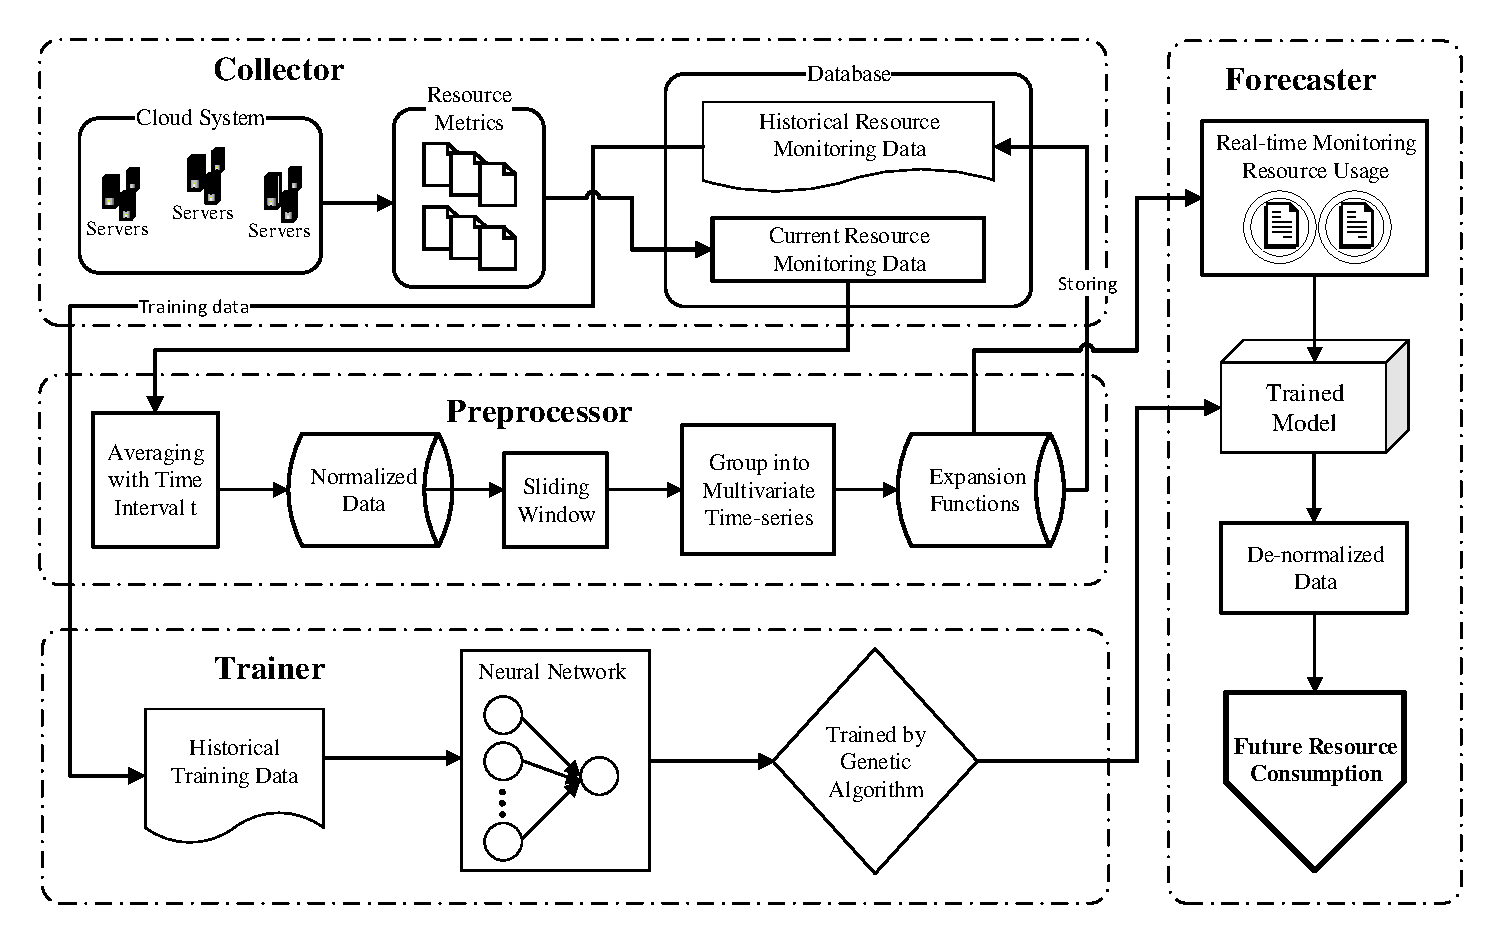
\includegraphics[scale=0.45]{FLGANN_system.pdf}
		\caption*{Proposed architecture of resources forecasting system}
		\label{fig:overall}
	\end{figure}
\end{frame}

\subsection{Preprocessor}
\begin{frame}{Preprocessor}
	\begin{figure}
		\centering
		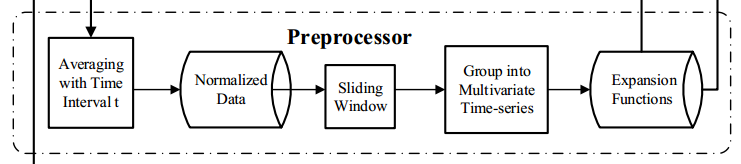
\includegraphics[width=0.75 \textwidth]{preprocessor.png} %[width=9cm,height=5cm]
		\label{fig:preprocessing}			
	\end{figure}
	\begin{itemize}
		\item{Construct suitable dataset for the learning part in our system }
		\begin{itemize}
			\item{\notesize Values of each cloud monitoring metric are transformed into the corresponding time series $r_i(t)$ ($i = 1, 2, \ldots, M$) with time interval $\tau$}
			\vspace{0.2cm}
			\item{\notesize Normalization, which scales a time series in the range of [0, 1]}
			\vspace{0.2cm}
			\item{\notesize Time-series data is transformed to supervised data by using sliding method.}
			\vspace{0.2cm}
			\item{\notesize Single multivariate data which is created by group all resource metric types.}
			\vspace{0.2cm}
			\item{\notesize Function Expansions such as Chebyshev, Legendre or Power help network has ability of catching the nonlinear relationship between the inputs and outputs.}
		\end{itemize}
	\end{itemize}
\end{frame}

\subsection{Trainer}
\begin{frame}{Trainer}

\begin{figure}
		\centering
		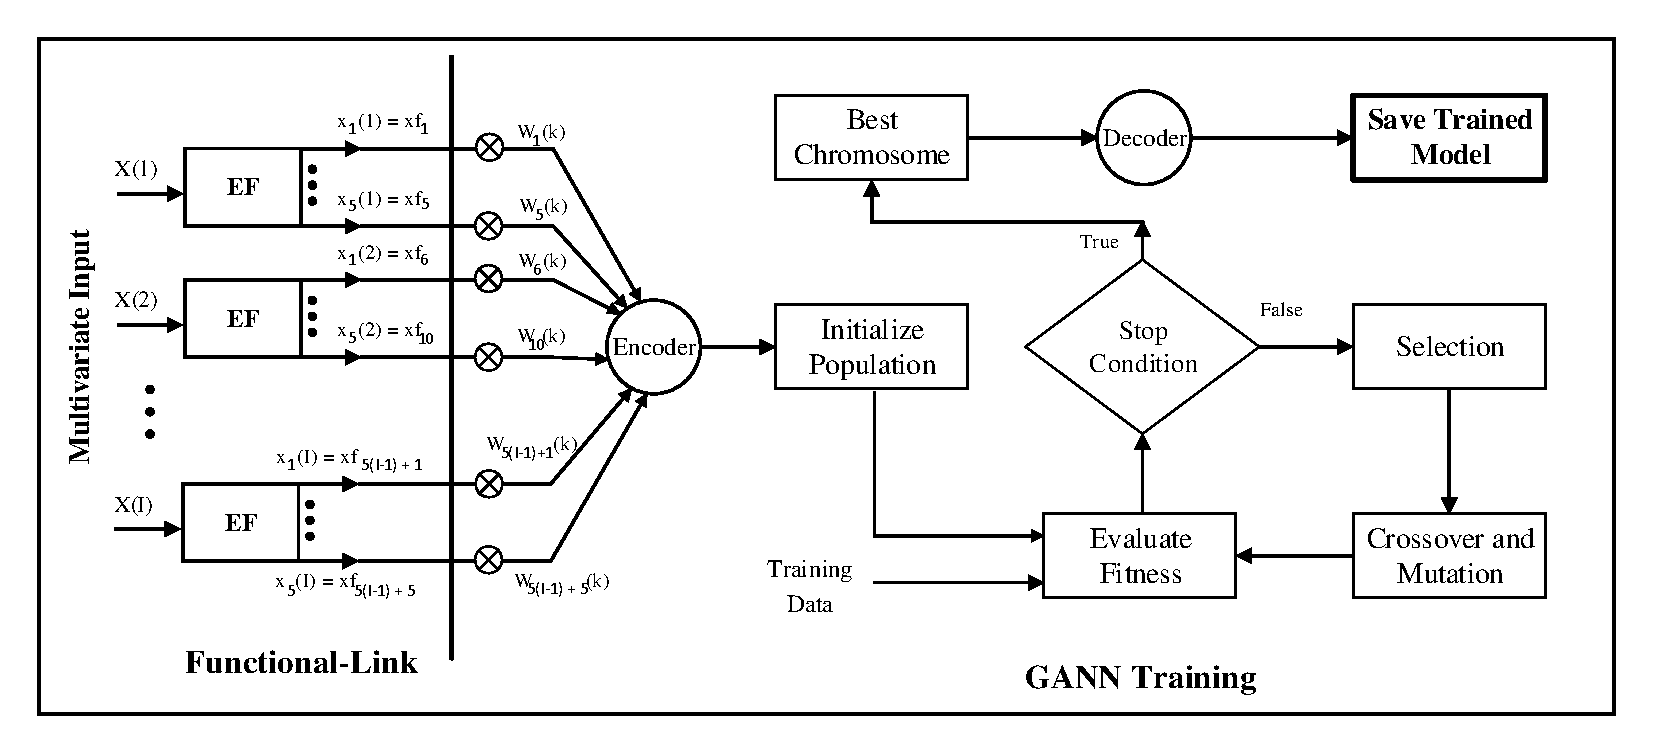
\includegraphics[width=0.8 \textwidth]{FLGANN_process.pdf} %[width=9cm,height=5cm]
		\caption*{\notesize Figure 1: FL-GANN training process}
		\label{fig:preprocessing}			
	\end{figure}
	\begin{itemize}
		\item{Figure 1 is FL-GANN training process}
		\begin{itemize}
			\item{\notesize Encoder component is used to encode the weights and bias of network into a chromosome (real-value vector). }
			\item{ \notesize Decoder component decodes the chromosome into the weights and bias of network. }
		\end{itemize}
	\end{itemize}
	
\end{frame}


\subsection{Forecaster}
\begin{frame}{Forecaster}
		\begin{itemize}
			\item The real-time monitoring resource usage will be preprocessing
			\item The trained model capture the logical fuzzy relationship: $F(t), F(t-1), F(t-2), \dots, F(t-p+1)) \rightarrow F(t+k)$
			\item The output value of trained model will be de-normalized into the real values.
		\end{itemize}

\end{frame}

\subsection{GA}
\begin{frame}{Genetic Algorithm}
	\begin{figure}
		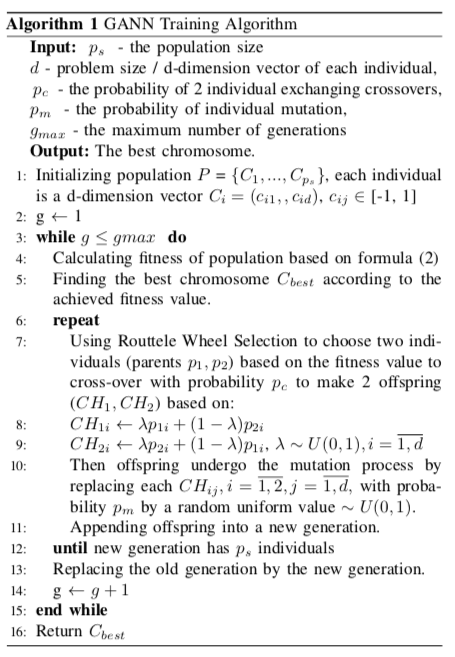
\includegraphics[width=0.45 \textwidth]{slide-GA-algo.png} %[width=9cm,height=5cm]
		\label{fig:ga}			
	\end{figure}
\end{frame}

\section{Experiments}
\subsection{Experimental setup}
\begin{frame}{Experimental setup}
	\frametitle{Experimental setup}
	\begin{itemize}
		\item {
			Data set: Google cluster trace dataset
			\begin{itemize}
			\item 20 metrics which are measured by several metrics such as CPU, memory usage, disk I/O mean time, and so forth
			\item 12O32799308 data items in data set
			\item  Less than 2\% of jobs that run longer than one day, even though such jobs contribute to over 80\% of the dataset records
			\item A long-running job with ID 6176858948 that consists of 25954362 monitoring data items during the 29-day period
			\item Used dataset from 1st to 20th day to train model and from 21st to 29th to evaluate the model performance.
			\end{itemize}
		}
		\item{
			The fitness function in GA: \newline
			$Fitness = \displaystyle \frac{1}{MAE} = \frac{N}{ \displaystyle \sum_{i=0}^N( forecast(i) - y_i)^2 }	\label{eq_fitness} $. 
			}
	\end{itemize}
\end{frame}


\subsection{Forecasting Resource Consumption}
\begin{frame}{Forecasting Resource Consumption}
\begin{notesize}
\begin{table}[h]
	\caption{MAE comparison of MLNN, traditional FLNN and FL-GANN models}
	\begin{center}
		\begin{tabu}{| c | c| c | c | c | c | c | c |}
			\hline
			\textbf{Input Type} & \textbf{Model} & \multicolumn{3}{c}{\textbf{CPU}}  & \multicolumn{3}{|c|}{\textbf{RAM}}  \\ \cline{3-8} 
			& & k = 2 & k = 3 & k = 5 & k = 2 & k = 3 & k = 5  \\ [0.5ex] \hline
			& MLNN & 0.3327	& 0.3514 & 0.3570	& 0.0288	& 0.0265 	& 0.0273  \\ 
			Univariate & FLNN	& 0.2944 	& 0.2999  & 0.3054	& 0.0210 	& 0.0201 	& 0.0215  \\
			& FL-GANN	& \textbf{0.2829}	& \textbf{0.2812} & \textbf{0.2843}	& \textbf{0.0195} 	& \textbf{0.0197}	& \textbf{0.0202}  \\ \hline
			
			& MLNN	& 0.3314	& 0.3387 	& 0.3448	& 0.0266 & 0.0271	& 0.0289 \\ 
			Multivariate & FLNN	& 0.2971 	& 0.2903 	& 0.3201	 & 0.0218  & 0.0202	& 0.0226   \\ 
			& FL-GANN	& \textbf{0.2815}	& \textbf{0.2814} 	& \textbf{0.2902}	& \textbf{0.0194} & 0.0207	& \textbf{0.0212}   \\ \hline 
		\end{tabu}
		\label{table:forecasting_results_MLNN_FLNN_FLGANN}
	\end{center}
\end{table}
\end{notesize}
\end{frame}


\begin{frame}{Forecasting}
	\begin{figure}
		\centering
		\begin{subfigure}{0.5\textwidth}
			\centering
			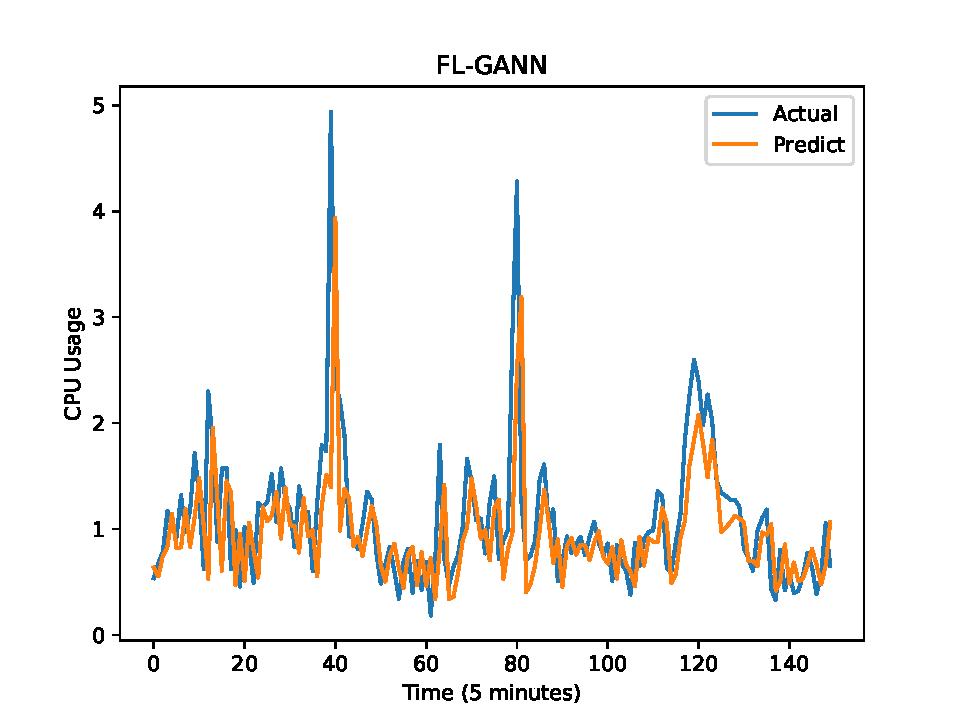
\includegraphics[width=1.0\linewidth]{multi_cpu_flgann.pdf}
			\label{fig:sub11}
		\end{subfigure}%
		\begin{subfigure}{.5\textwidth}
			\centering
			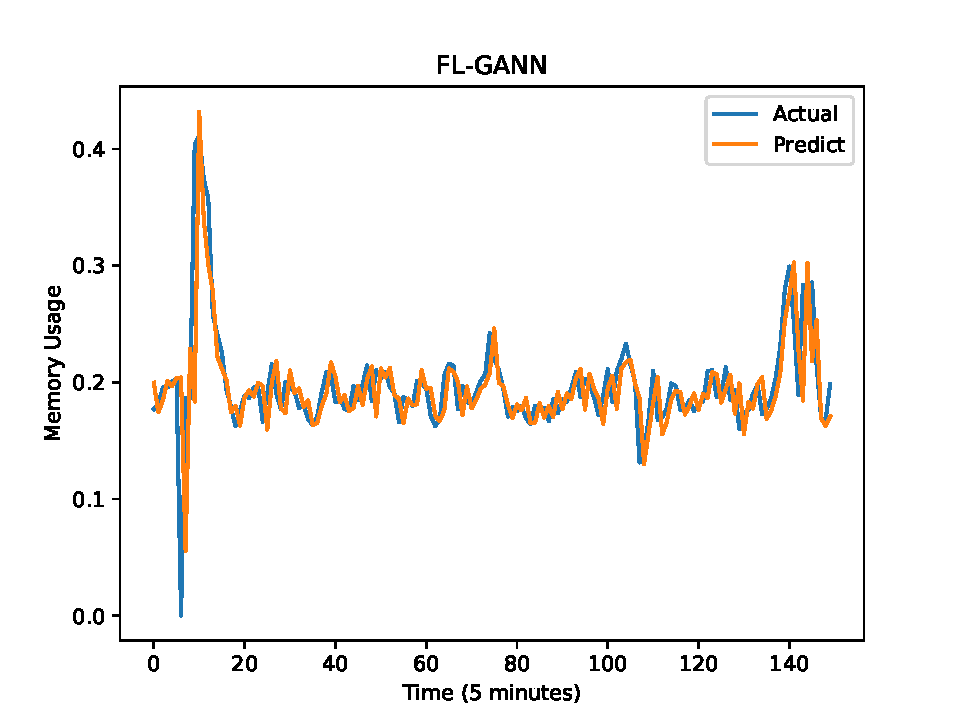
\includegraphics[width=1.0\linewidth]{multi_ram_flgann.pdf}
			\label{fig:sub21}
		\end{subfigure}%
		\caption{CPU usage and Memory usage of FL-GANN models}
		\label{fig:cpu_predict}
	\end{figure}

\end{frame}



\subsection{Influence of GA hyper-parameter on FL-GANN}
\begin{frame}{Population size changing experiment}
	\begin{figure}
		\centering
		\begin{subfigure}{0.4\textwidth}
			\centering
			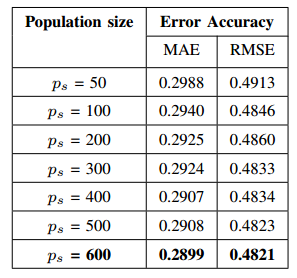
\includegraphics[width=1.0\linewidth]{ps_changing.png}
			\caption*{\notesize Comparison of average MAE and RMSE with different population sizes}
			\label{fig:sub11}
		\end{subfigure}%
		\begin{subfigure}{.6\textwidth}
			\centering
			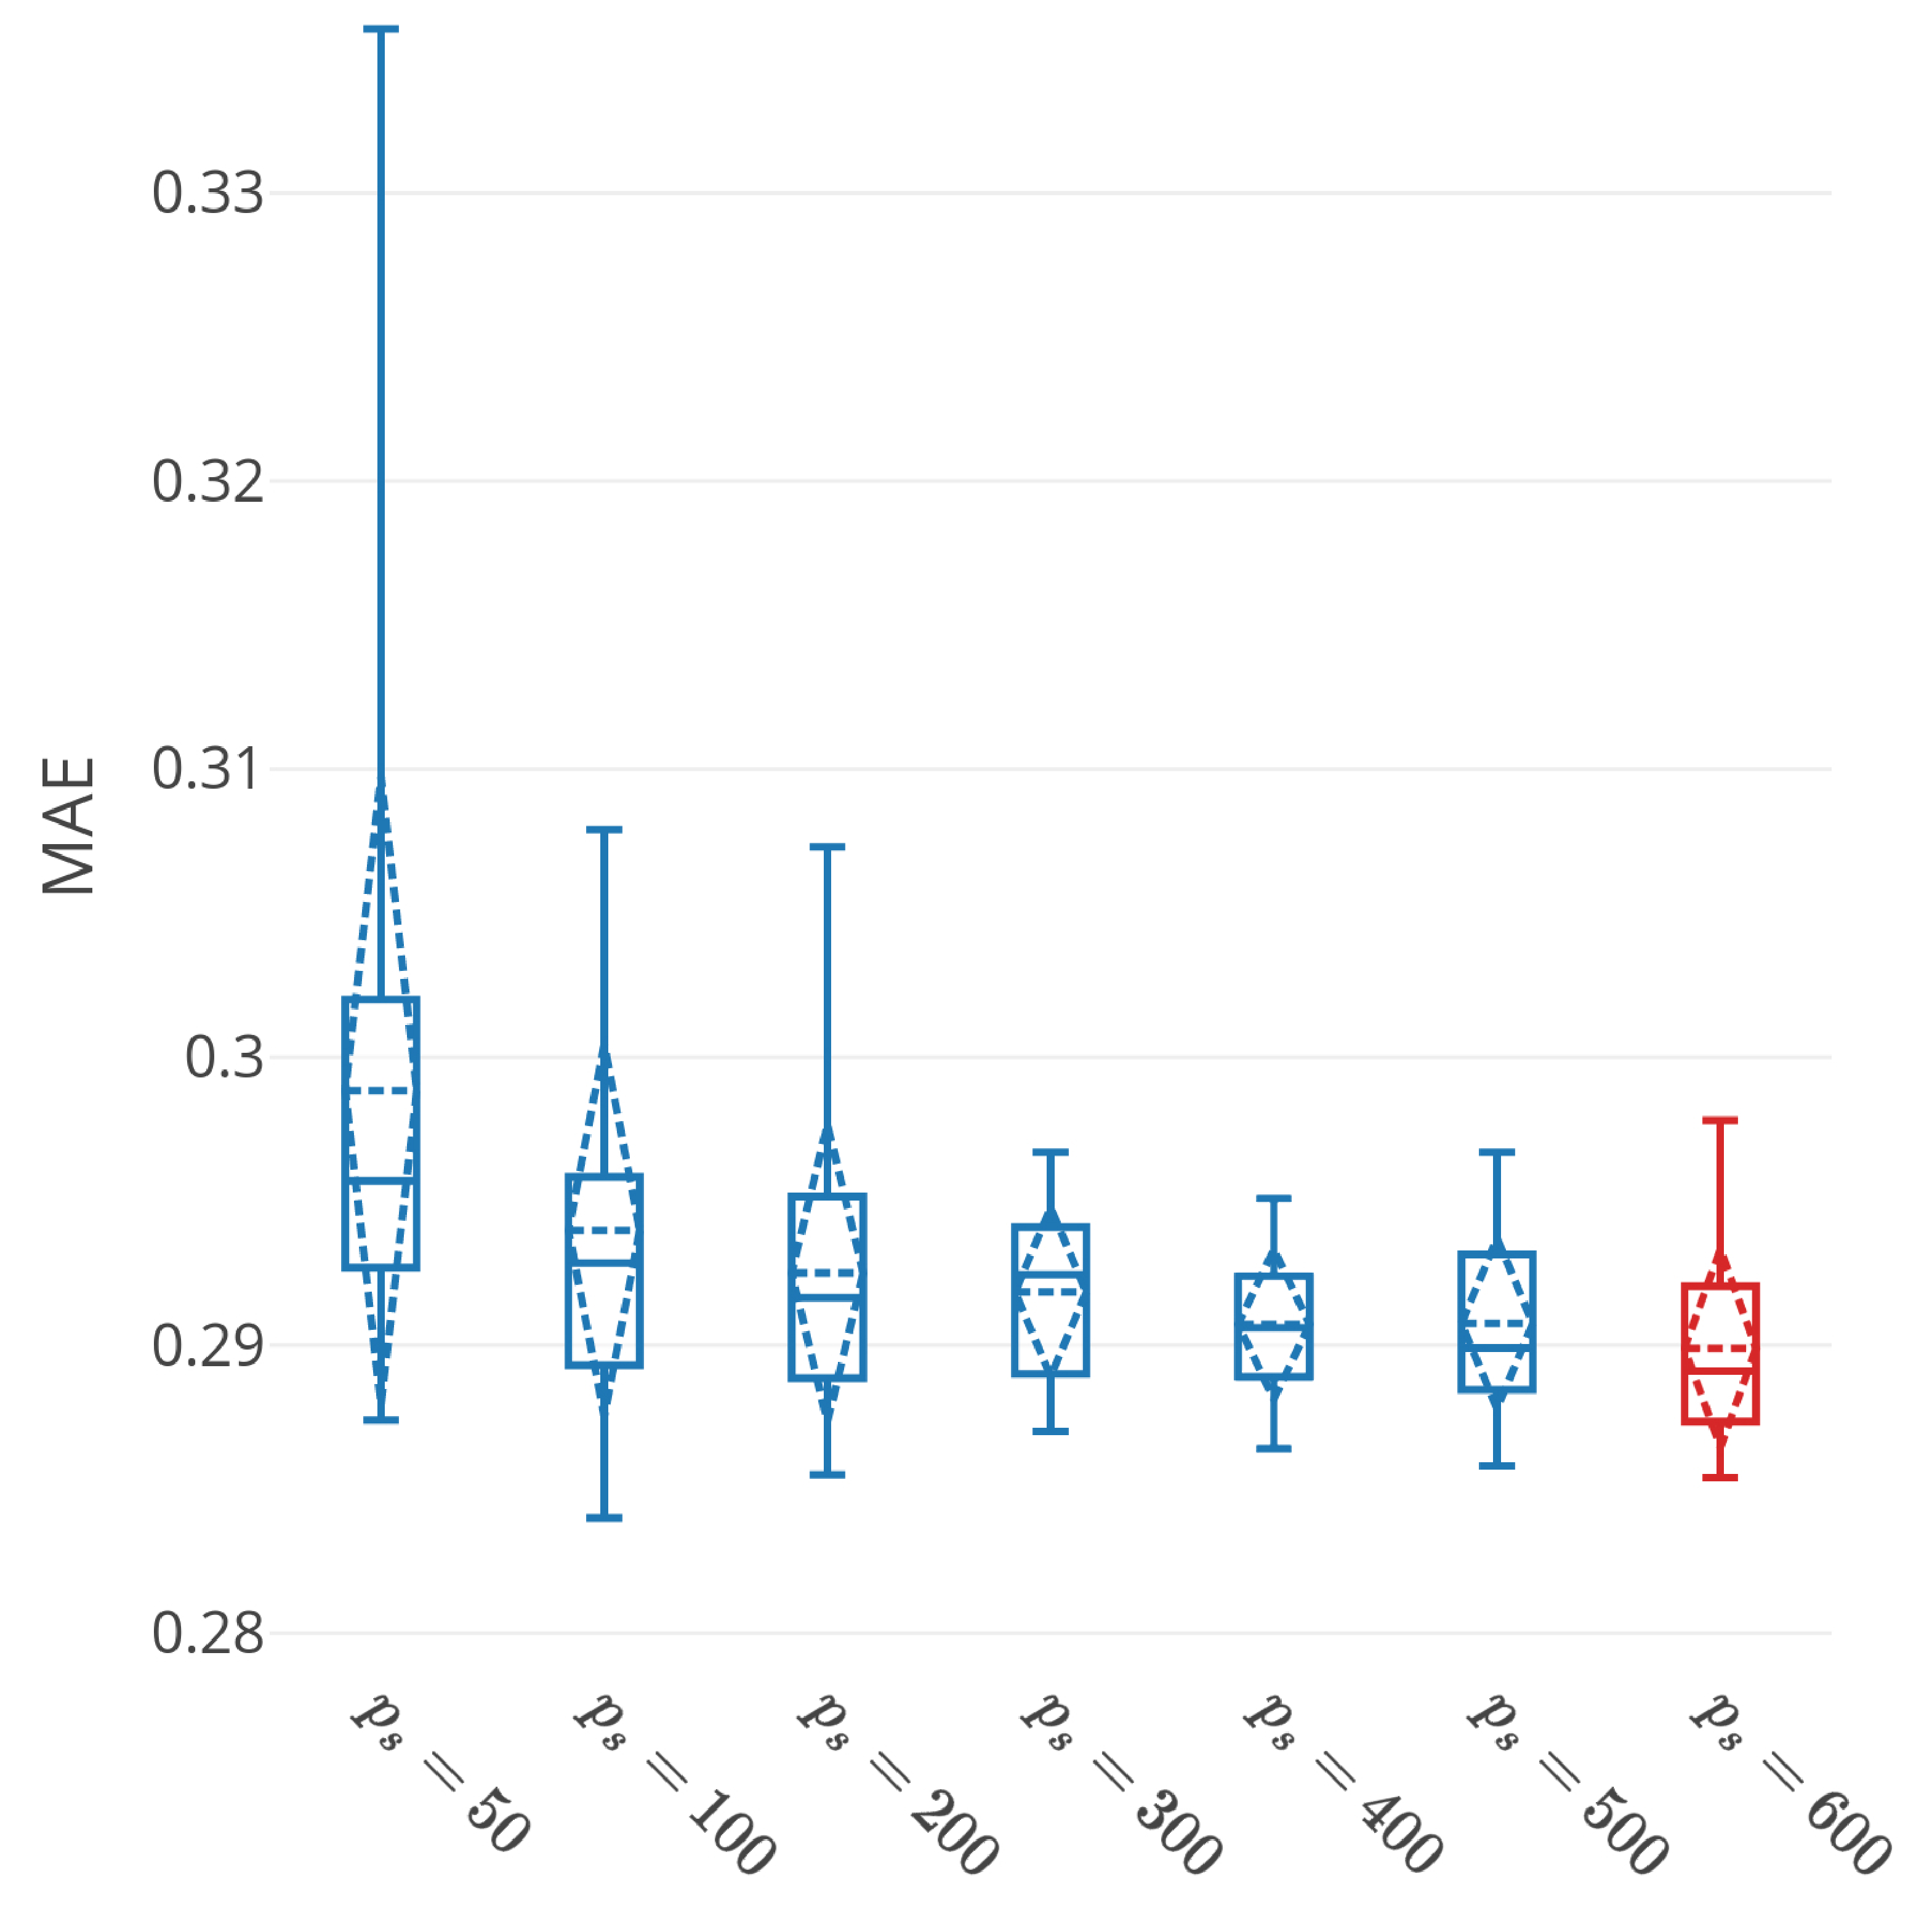
\includegraphics[width=0.8\linewidth]{tn2_multi_cpu_best_ps.pdf}
			\caption*{ \notesize MAE accuracy fluctuation comparison of with different population sizes}
			\label{fig:sub21}
		\end{subfigure}%
		\label{fig:cpu_predict}
	\end{figure}
\end{frame}

\begin{frame}{Probability of two individual exchanging crossover changing experiment}
	\begin{figure}
		\centering
		\begin{subfigure}{0.4\textwidth}
			\centering
			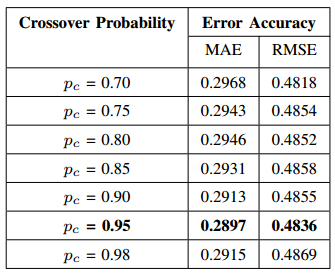
\includegraphics[width=1.0\linewidth]{pc_changing.png}
			\caption*{\notesize Comparison of average MAE and RMSE with different probability of two individuals exchanging crossovers}
			\label{fig:sub11}
		\end{subfigure}%
		\begin{subfigure}{.6\textwidth}
			\centering
			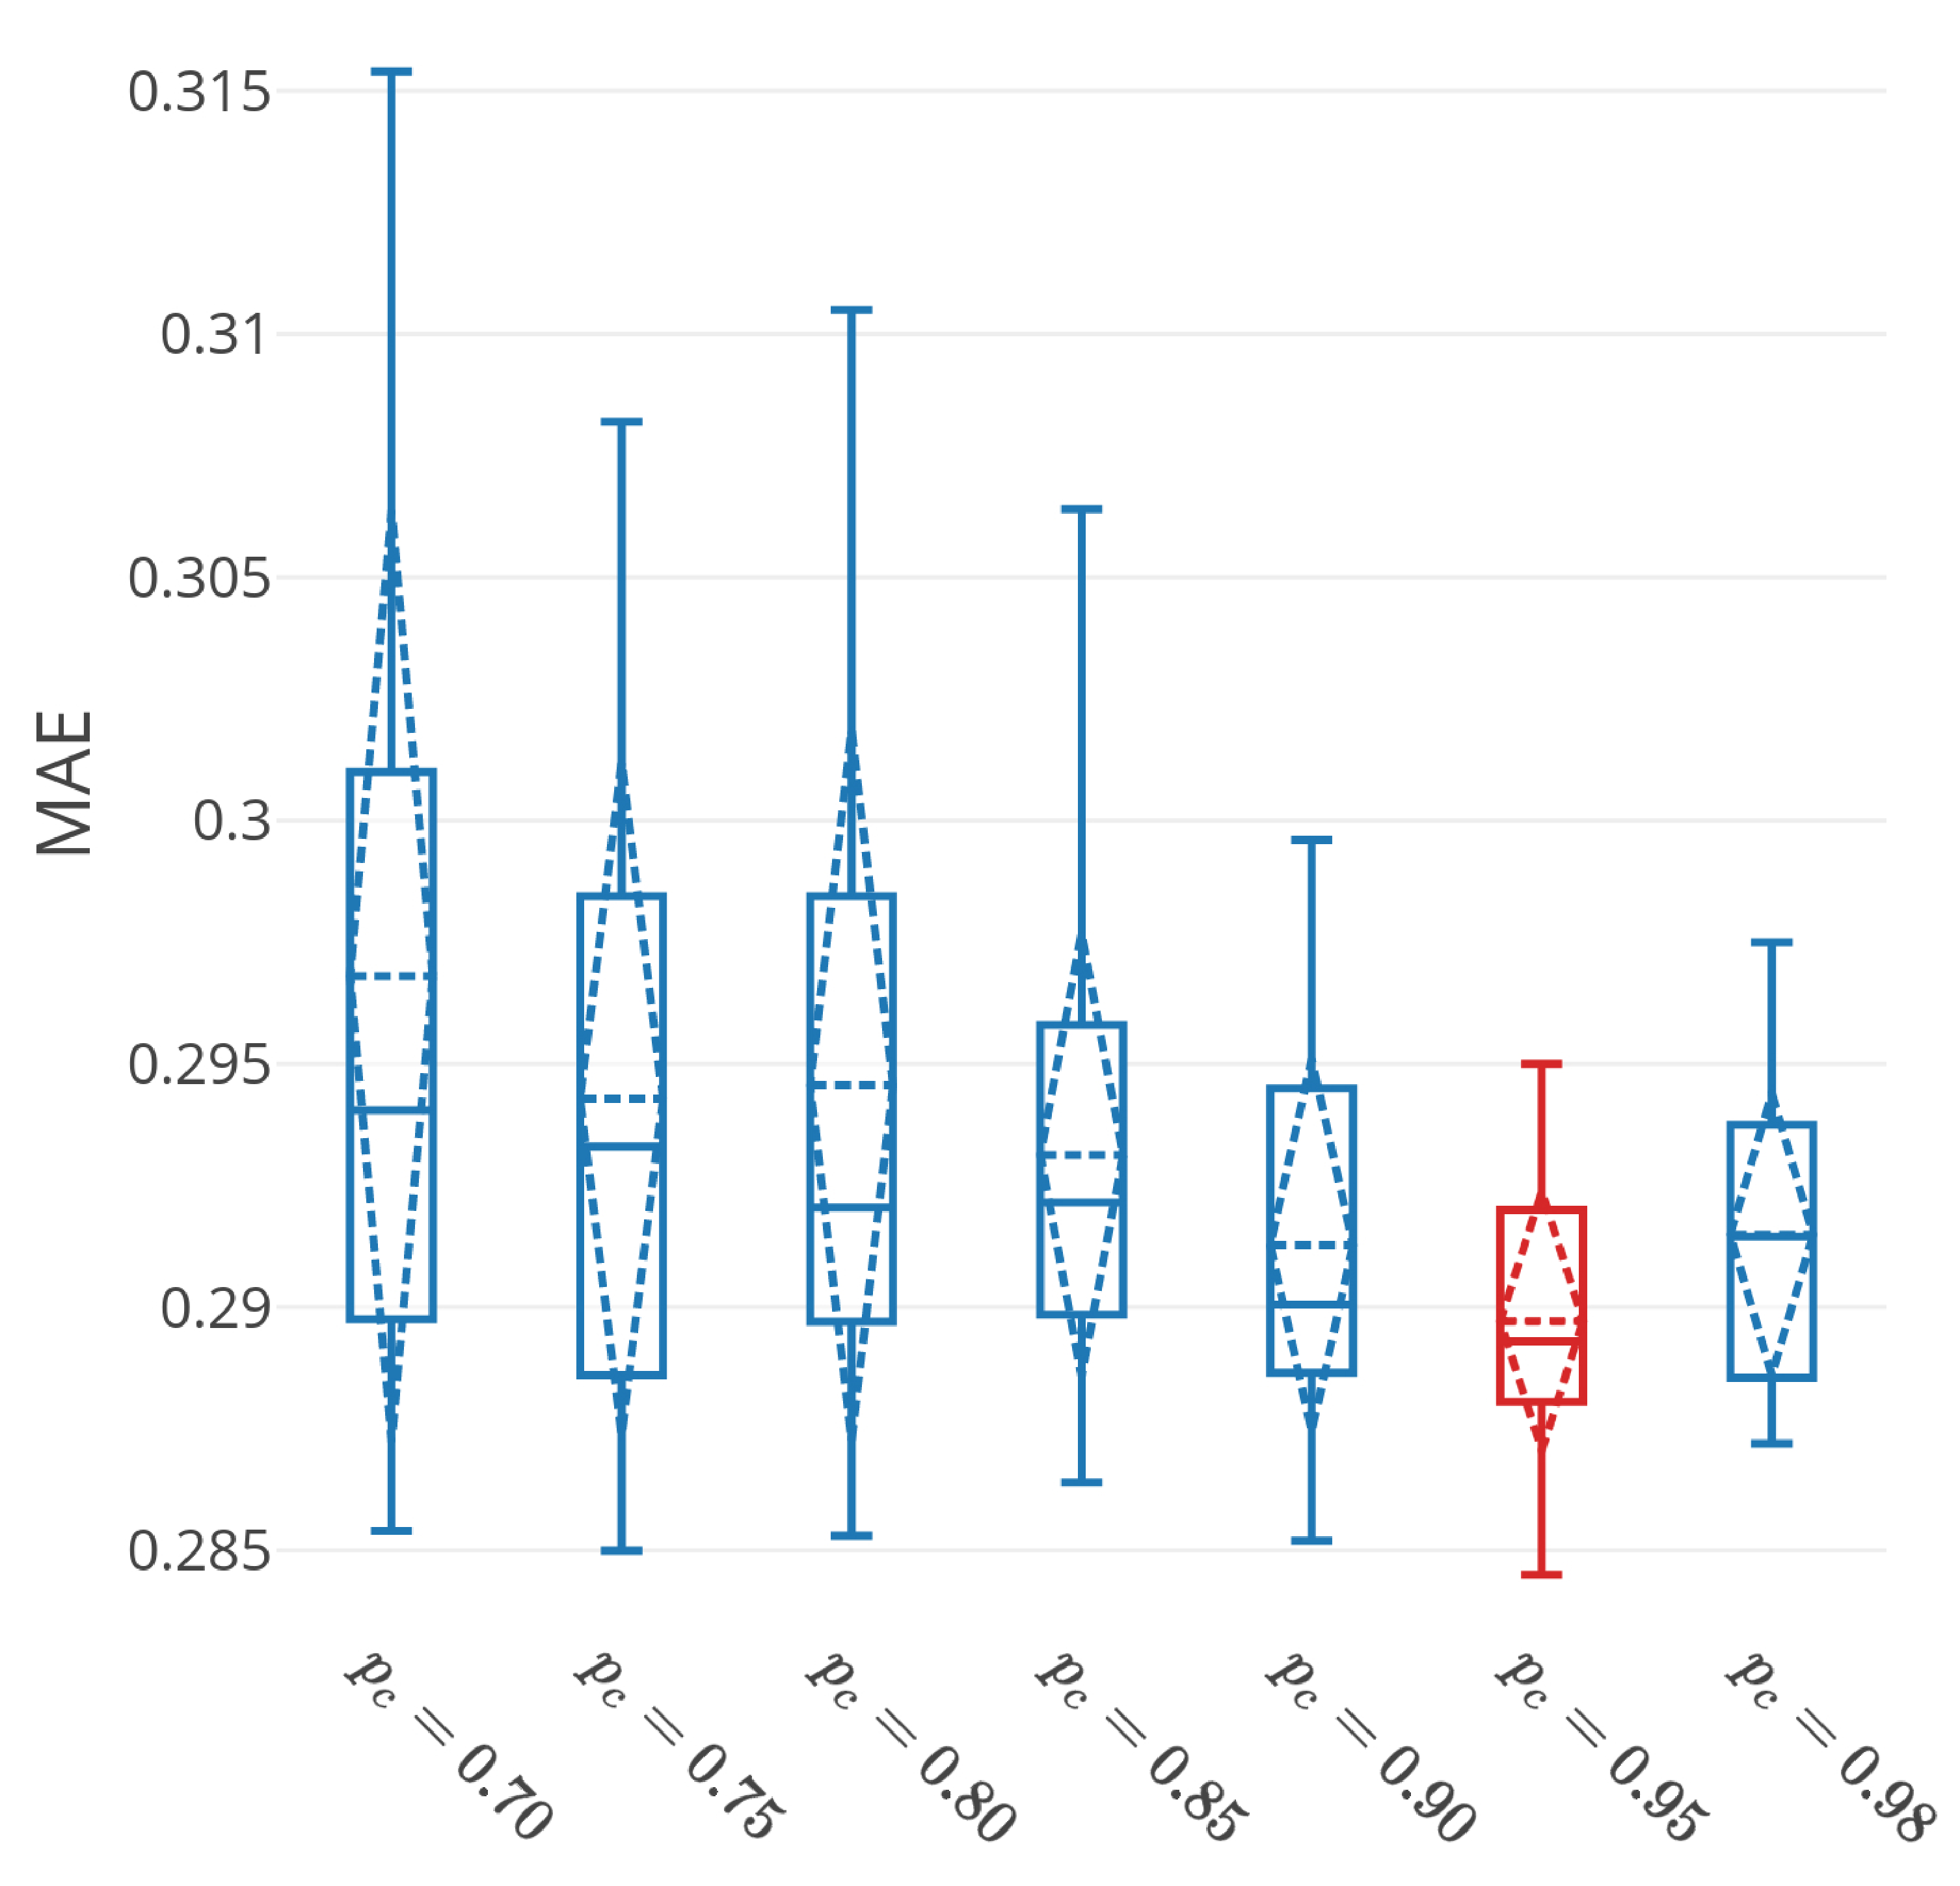
\includegraphics[width=0.8\linewidth]{tn2_multi_cpu_best_pc.pdf}
			\caption*{ \notesize MAE accuracy fluctuation comparison with different probability of two individuals exchanging crossovers}
			\label{fig:sub21}
		\end{subfigure}%
		\label{fig:cpu_predict}
	\end{figure}
\end{frame}


\begin{frame}{Probability of individual mutation changing experiment}
	\begin{figure}
		\centering
		\begin{subfigure}{0.4\textwidth}
			\centering
			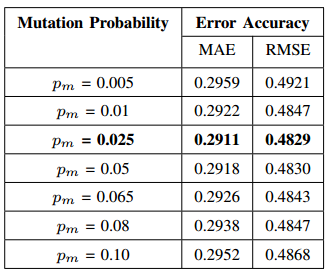
\includegraphics[width=1.0\linewidth]{pm_changing.png}
			\caption*{\notesize Comparison of average MAE and RMSE with different probability of individual mutation}
			\label{fig:sub11}
		\end{subfigure}%
		\begin{subfigure}{.6\textwidth}
			\centering
			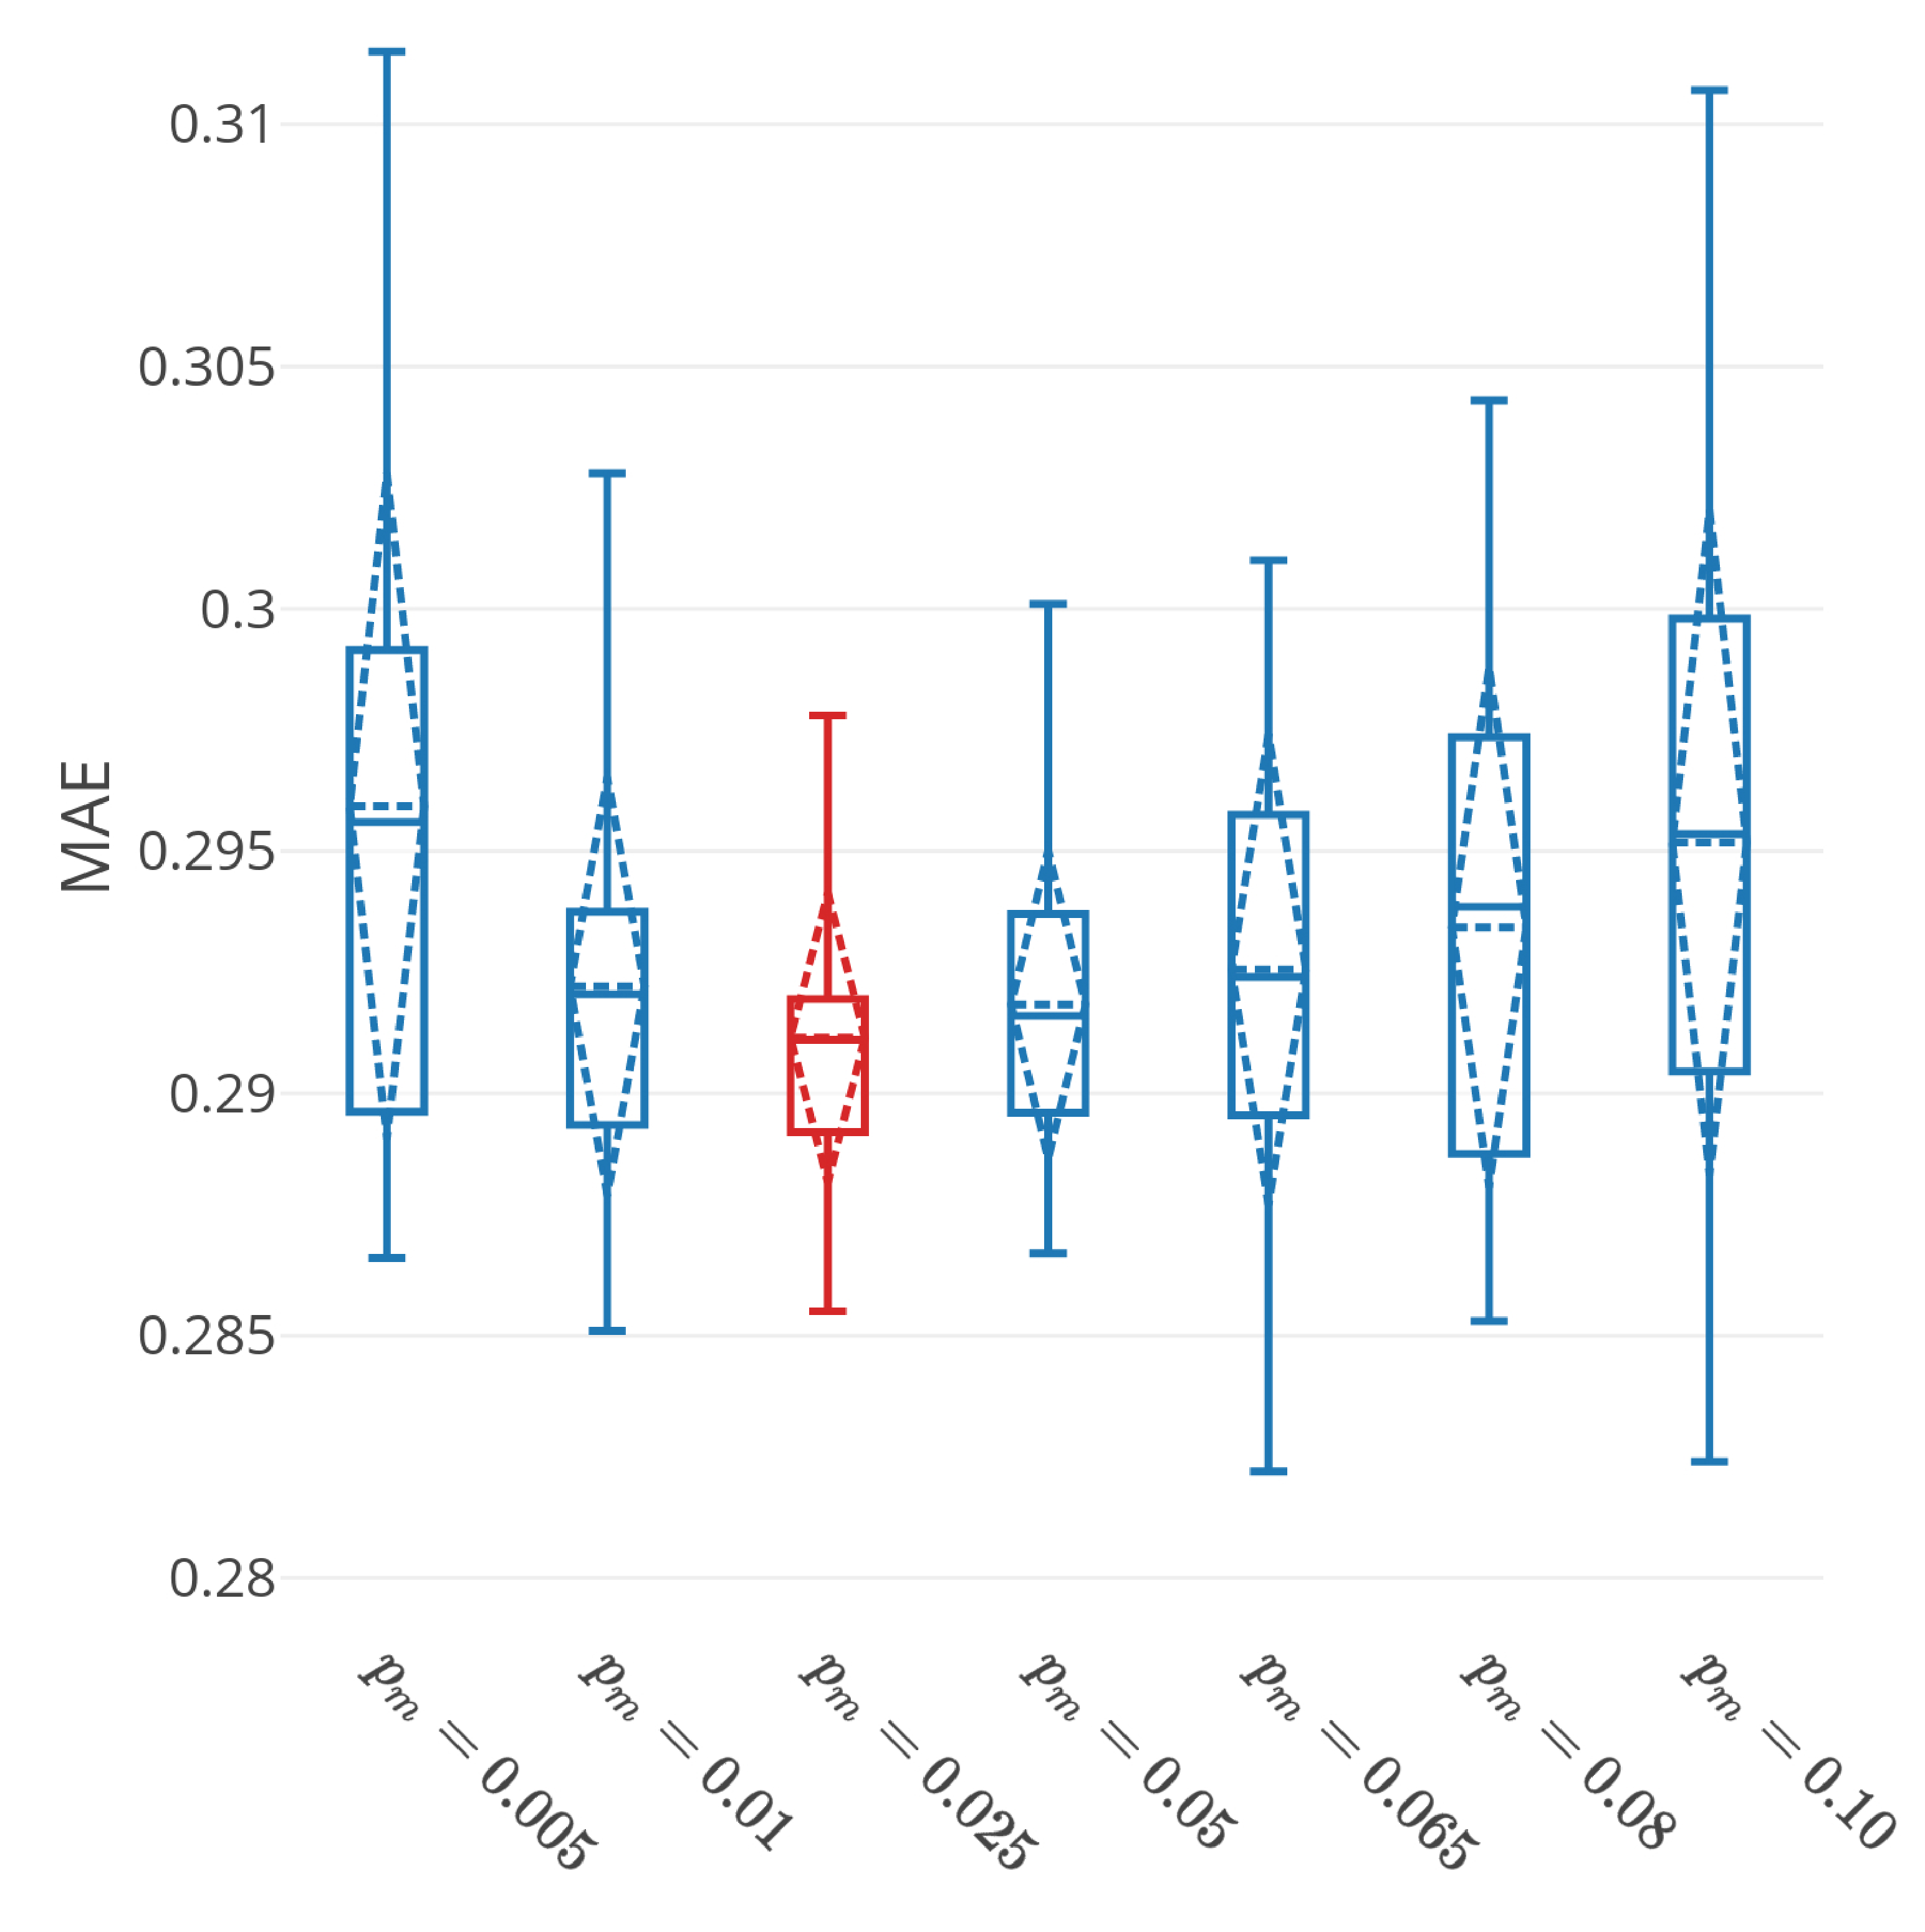
\includegraphics[width=0.8\linewidth]{tn2_multi_cpu_best_pm.pdf}
			\caption*{\notesize MAE accuracy fluctuation comparison with different probability of individual mutation}
			\label{fig:sub21}
		\end{subfigure}%
		\label{fig:cpu_predict}
	\end{figure}
\end{frame}


\subsection{Influence of Expansion Functions on FL-GANN}

\begin{frame}{Influence of Expansion Functions on FL-GANN}
	\begin{figure}
		\centering
		\begin{subfigure}{0.6\textwidth}
			\centering
			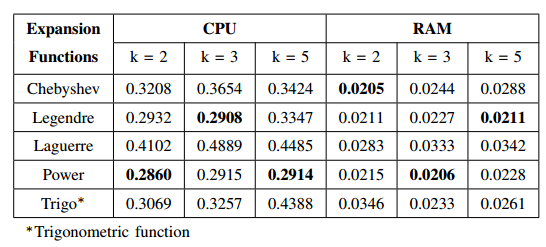
\includegraphics[width=1.0\linewidth]{expansion_function.png}
			\caption*{\notesize Comparison of average MAE and RMSE with different probability of two individuals exchanging crossovers}
			\label{fig:sub11}
		\end{subfigure}%
		\begin{subfigure}{.4\textwidth}
			\centering
			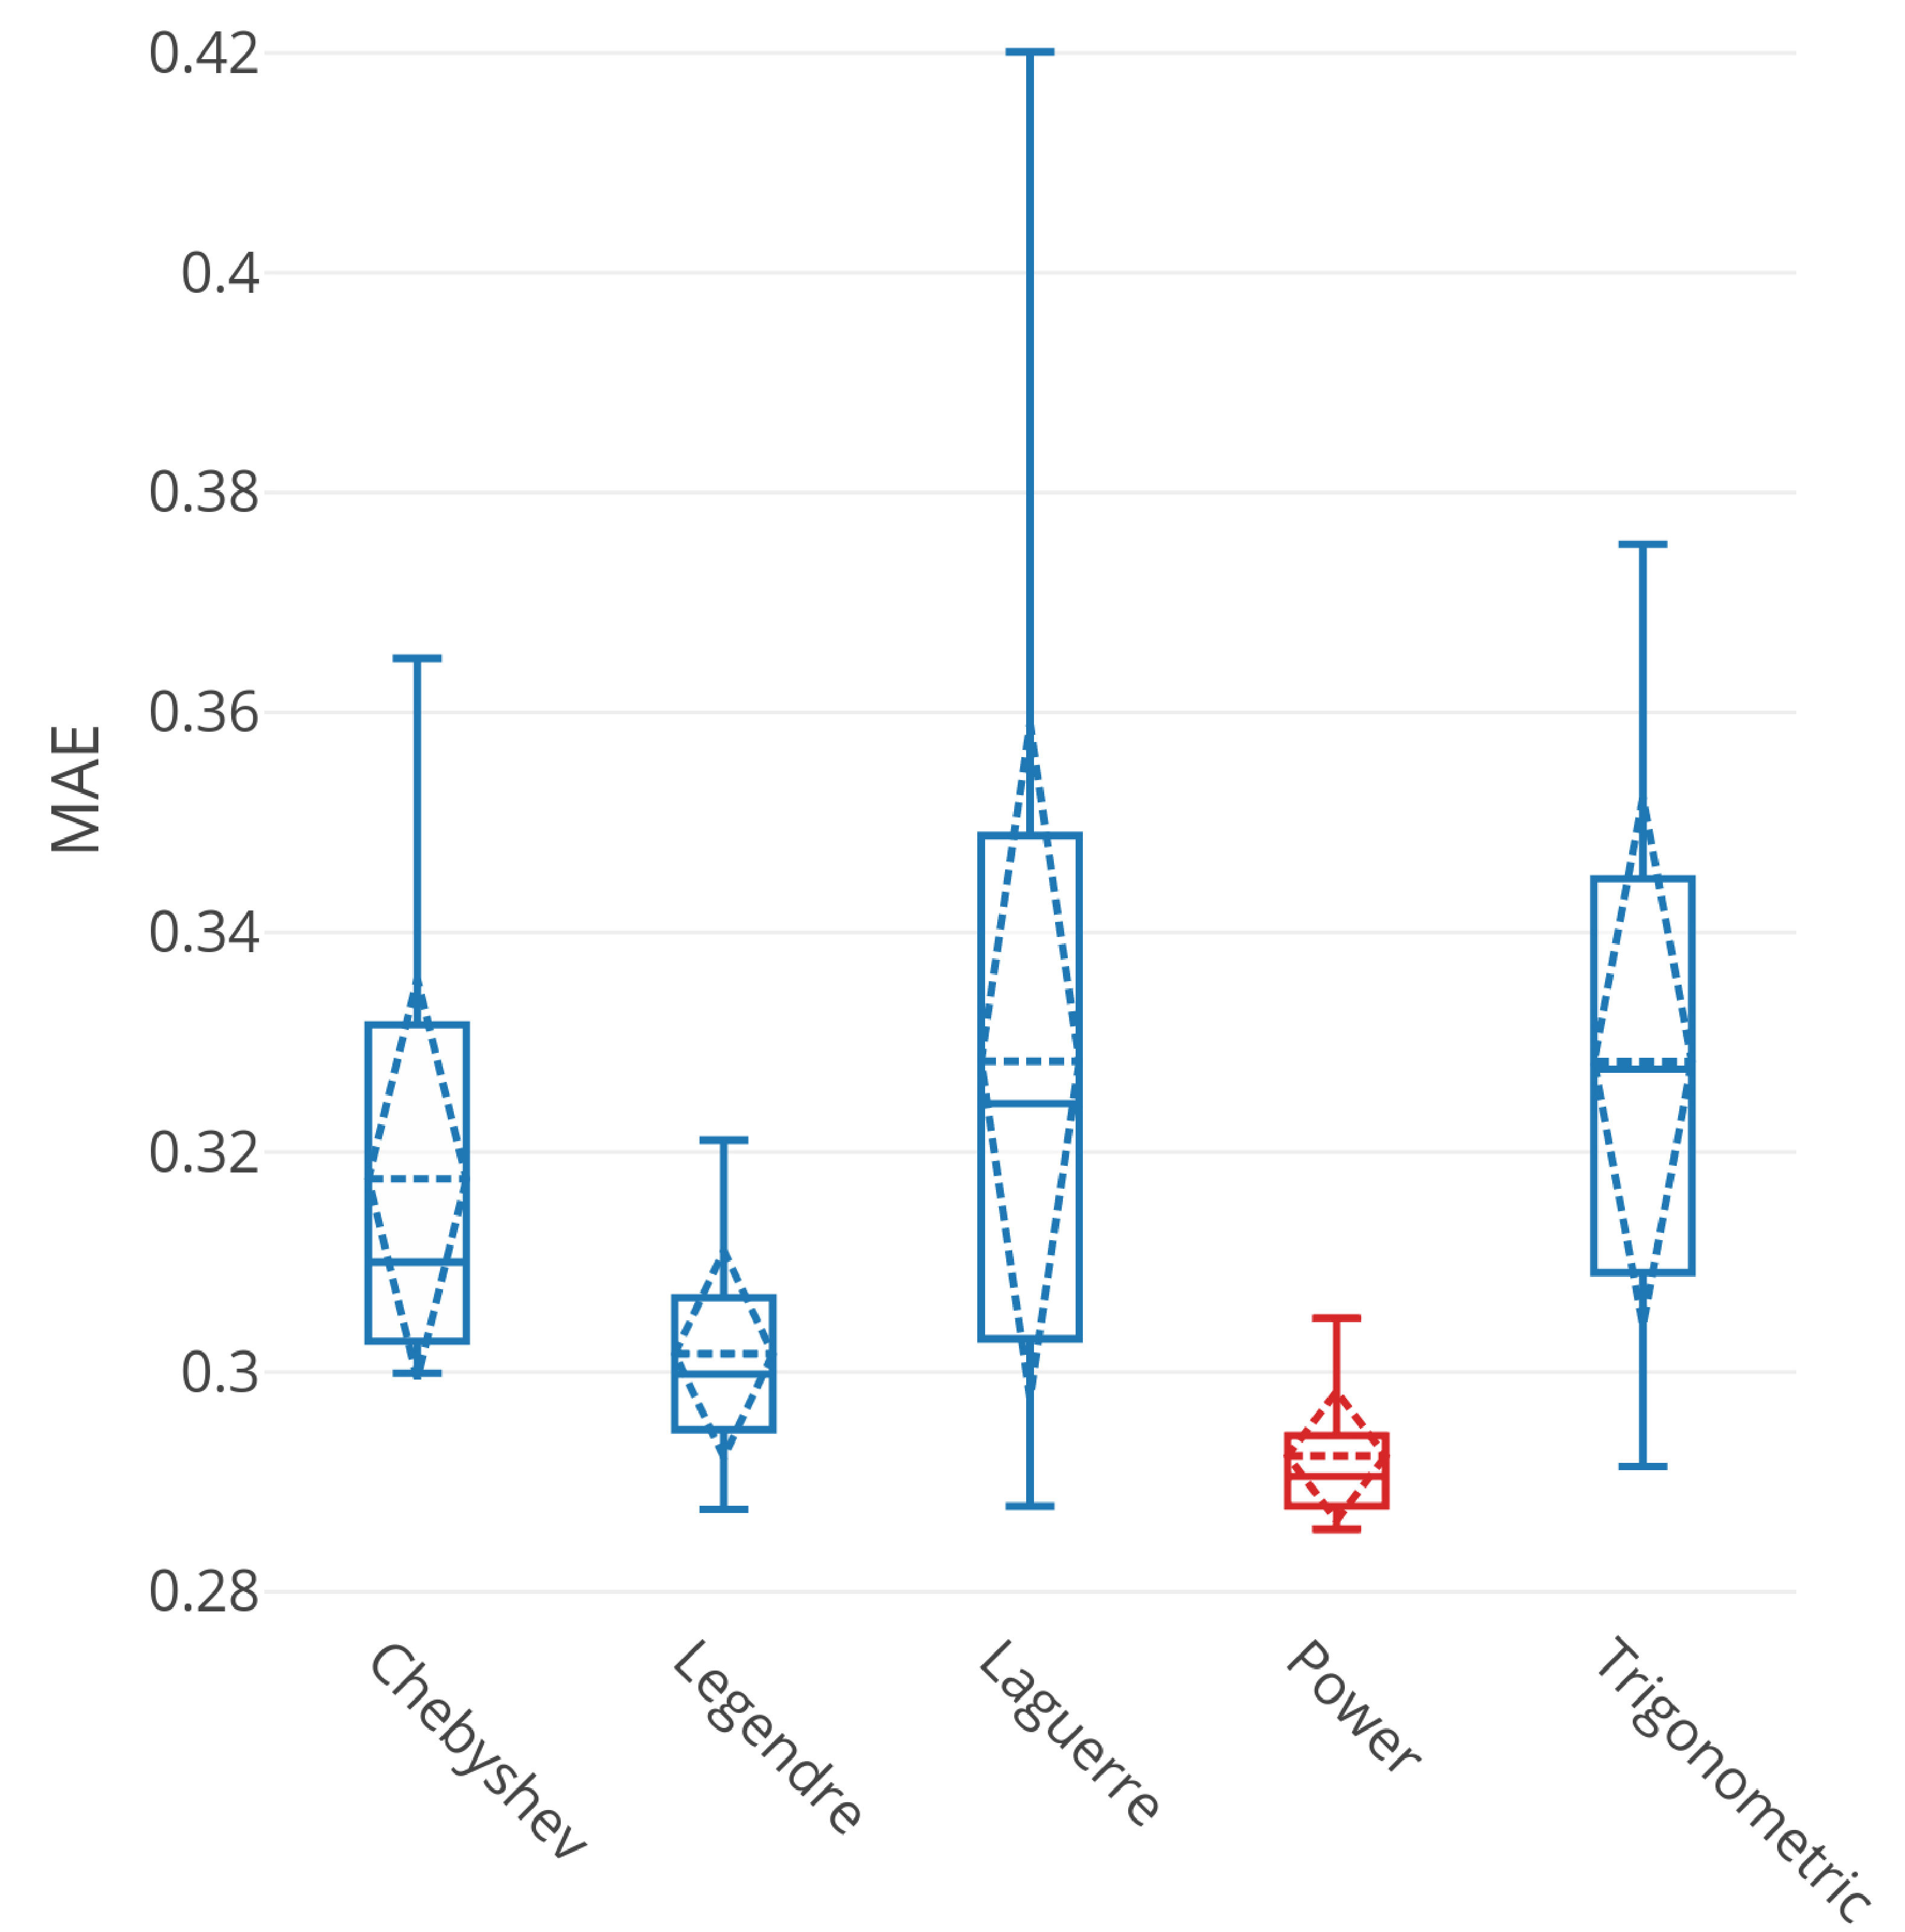
\includegraphics[width=1.0\linewidth]{tn2_multi_cpu_function.pdf}
			\caption*{\notesize MAE accuracy fluctuation comparison with different probability of individual mutation}
			\label{fig:sub21}
		\end{subfigure}%
		\label{fig:cpu_predict}
	\end{figure}
\end{frame}


\section{Conclusion and future work}
\begin{frame}{Conclusion and future work}
	\begin{itemize}
		\item {
		Proposed a new prediction system with experiments for cloud proactive auto-scaling service focusing on exploiting multivariate monitoring data
		}
		\item{
			Several mechanisms to improve accuracy as well as effectiveness of the resource usage prediction model using
			\begin{itemize}
			\item {
				Functional-link Neural Network (FLNN)
			}
			\item {
				Genetic Algorithm (GA) to train the FLNN instead of traditional BP (called FL-GANN)
			}
			\item{
				Analyze the influence of GA parameters and FLNN to FL-GANN
			}
		\end{itemize}
		}
	\end{itemize}
\end{frame}

\begin{frame}{}
	
		\centering \Huge
		\emph{Thank you for your attention!!!}
		\emph{Q\&A}
			
		
\end{frame}
%\label{sect:bib}
%\bibliographystyle{plain}
%\bibliography{reference}
\end{document}


